\documentclass[]{IEEEtran}

\title{Ottimizzazione distribuita di sintesi hardware tramite approccio map-reduce con framework Hadoop}
\author{Andrea Caucchiolo - VR436780\\Elia Brentarolli - VR433534}

\usepackage{graphicx}
\usepackage[english,italian]{babel}
\usepackage[utf8]{inputenc}
\usepackage{caption}
\usepackage{amsmath}
\usepackage{longtable,array,booktabs}
%\usepackage{hyperref}
\usepackage{uri}
\usepackage{xcolor}
%\usepackage{textcomp}
\usepackage{graphics}
\usepackage{listings}
\usepackage[ center ]{ subfigure }
\definecolor{dkgreen}{rgb}{0,0.6,0}
\definecolor{gray}{rgb}{0.5,0.5,0.5}
\definecolor{mauve}{rgb}{0.58,0,0.82}
\lstdefinestyle{javaStyle}{
	language=Java,
	aboveskip=3mm,
	belowskip=3mm,
	showstringspaces=false,
	columns=flexible,
	basicstyle={\small\ttfamily},
	numbers=none,
	numberstyle=\color{black},
	keywordstyle=\color{blue},
	commentstyle=\color{dkgreen},
	stringstyle=\color{mauve},
	breaklines=true,
	breakatwhitespace=true,
	tabsize=3,
	escapechar=^
}

\usepackage{fancyvrb}

% redefine \VerbatimInput
\RecustomVerbatimCommand{\VerbatimInput}{VerbatimInput}%
{fontsize=\footnotesize,
	%
	frame=lines,  % top and bottom rule only
	framesep=2em, % separation between frame and text
	rulecolor=\color{gray},
	%
	commandchars=\|\(\), % escape character and argument delimiters for
	% commands within the verbatim
	commentchar=*        % comment character
}
\begin{document}
\maketitle

\begin{abstract}
	
Questo documento contiene una relazione sullo sviluppo di un programma per ottimizzare la sintesi hardware partendo dal \emph{control flow graph} di un software tramite un  approccio di tipo map-reduce e sfruttando al massimo le capacità di calcolo distribuito offerte dal framework Hadoop. In particolare il programma proposto, preso in input un \emph{control flow graph} del software da sintetizzare e il livello di parallelismo voluto, detto $n$, produce in output $n$ grafi temporizzati scelti tra quelli che rendono minima la funzione di costo definita nel programma stesso.

\end{abstract}


\section{Introduzione}

La possibilità di generare in modo automatico la descrizione di una piattaforma hardware che esegue le stesse operazioni di un software partendo dallo stesso è, ad oggi, una tecnica ancora troppo imprecisa e inaffidabile per poter essere impiegata su larga scala. In particolare per poter approcciarsi a questa tecnica è necessario, tra le varie problematiche, affrontare un problema di ricerca della migliore combinazione dei nodi di un grafo tra tutte le varie permutazioni possibili dello stesso. Ovviamente la risoluzione di un problema del genere per grafi con milioni di permutazioni richiede delle risorse di tempo troppo elevate perché questo possa essere fatto su una singola macchina. Proprio per questo motivo si è deciso di proporre un algoritmo risolutivo basato su cluster computing e, quindi, di andare ad abbattere le tempistiche eseguendo le computazioni su più macchine in modo da poter ottenere risultati di istanze troppo complesse per in tempi non troppo elevati. Inoltre l'approccio distribuito, a differenza della singola macchina, è molto più scalabile e quindi potenziabile per ottenere risultati sempre migliori a problemi sempre più complessi andando a mantenere tuttavia il costo per l'implementazione relativamente basso.

\section{Conoscenze preliminari e terminologia usata}

Per avere una migliore comprensione della relazione di seguito sono riportati alcuni concetti chiave le relative spiegazioni:
\begin{itemize}
	\item \textbf{High Level Synthesis} (HLS) \cite{HLS}: La sintesi ad alto livello è un'insieme di procedure che permettono di passare da un software scritto in un linguaggio ad alto livello alla descrizione di una piattaforma hardware in grado di eseguire le stesse operazioni del software di partenza e rispettando al contempo i vincoli imposti sulla velocità delle operazioni, le dimensioni del chip e il costo per la produzione. La figura \ref{hls} mostra i passaggi chiave della procedura. Nel corso della relazione si farà riferimento solamente alla fase di scheduling in quanto rappresenta la parte più difficile da affrontare.
	\begin{figure}[htp]
		\centering
		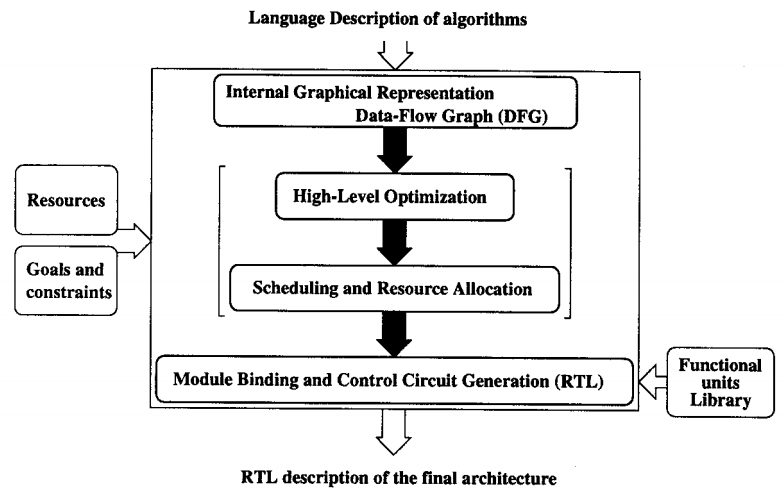
\includegraphics[width=0.5\textwidth]{images/Hls_flow.png}
		\caption{Schema del processo di \emph{high level synthesis}}
		\label{hls}
	\end{figure}
	
	\item \textbf{Data Flow Graph}: In questa relazione un \emph{data flow graph }rappresenta un grafo ottenuto partendo dall'analisi di un software generico e che contiene le informazioni sulle dipendenze delle operazioni e sulle componenti che devono essere usate. Qui un Data Flow Graph è definito formalmente come:
	\it{DFG} \normalfont $=(V,E)$ dove $\forall v_i\in V : v_i = (n,o)$ con $n$ rappresentante il nome del nodo, \emph{univoco} all'interno del grafo, e $o$ rappresentante invece il tipo di operazione che il nodo esegue (somma, divisione, operatori logici etc.). Infine si ha che $E = {(v_i,v_j)}, v_i,v_j \in V$ tali che $(v_i,v_j) \in E \iff v_j$ dipende da $v_i$ ovvero $v_j$ usa un risultato prodotto dalla computazione di $v_i$. Si vuole infine sottolineare che per come è stato definito un DFG non è possibile avere cicli nel grafo poiché ciò implicherebbe una dipendenza ciclica tra le istruzioni del software di partenza, indicando l'incorrettezza dello stesso.
	
	\item \textbf{Grafo temporizzato}: Durante la relazione si farà più volte accenno al concetto di \emph{grafo temporizzato} ottenuto dalla elaborazione di un DFG. Un grafo temporizzato non è altro infatti che un DFG arricchito con delle informazioni sulla tempistica delle operazioni, ovvero il tempo minimo e massimo ai quali l'operazione contenuta nel nodo può essere fatta senza che si sovrapponga a quelle dei propri padri o figli. Formalmente si ha:
	\it{TG} \normalfont $=(V,E)$ con $\forall v_i\in V : v_i = (n,o,t,T,m)$, dove $n,o$ hanno lo stesso significato che hanno nella definizione del DFG, $t$ rappresenta il tempo \emph{minimo} in cui l'operazione può essere fatta, $T$ rappresenta invece il tempo \emph{massimo} in cui l'operazione può essere svolta e $m$ rappresenta la mobilità del nodo nel tempo rispetto a $t$, ovviamente mantenendo sempre $m+t\le T$. Vale inoltre che $T - t = m$. L'insieme $E$ è definito invece in modo del tutto analogo a come fatto con DFG ma con la conseguenza che deve valere $\forall (v_i,v_j) \in E : t(v_i)<t(v_j) \land T(v_i)<T(v_j)$.
	Infine si dice che un grafo temporizzato è una \emph{permutazione} di un'altro grafo se per ogni nodo del primo grafo esiste un corrispettivo nodo nel secondo che differisce esclusivamente per il valore di $m$
	
	\item \textbf{Map-Reduce}\cite{MAPRED}: Paradigma di programmazione per il calcolo distribuito, consiste nel dividere un input di grandi dimensioni i diverse porzioni che vengono poi processate tutte in modo indipendente dalle altre (map). In seguito i risultati parziali vengono raccolti, ordinati e redistribuiti tra le macchine in base al valore impostato come chiave (shuffle and sort) per poi essere combinati nei risultti finali (reduce). La figura \ref{mapred} schematizza il processo appena descritto.
	\begin{figure}[htp]
		\centering
		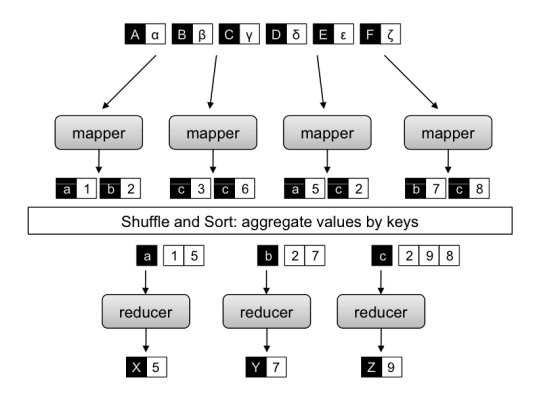
\includegraphics[width=0.5\textwidth]{images/mapred.png}
		\caption{Schema del processo di map-reduce. L'input è diviso tra i vari mapper che producono una serie di risultati del tipo chiave-valore. Successivamente i risultati sono raccolti e ridivisi tra i reducer in base al valore della loro chiave.}
		\label{mapred}
	\end{figure}
	
	\item \textbf{Hadoop} \cite{HADOOP}: Framework di Apache per Java per il calcolo distribuito e che si presta molto bene per l'approccio di tipo map-reduce. Sebbene il framework sia costituito da svariate componenti quali ad esempio l'Hadoop Distributed File System (HDFS) e molto altro, per la comprensione di questa relazione è necessario conoscere solo le classi principali riguardanti l'approccio map-reduce e che verranno spiegate nel dettaglio nel seguito della relazione.
\end{itemize}

\section{Definizione del problema affrontato}
Per poter capire meglio il problema che ci si è posto è necessario prima di tutto spigare molto brevemente in cosa consiste il flusso di progettazione di un sistema embedded (si prenda la figura \ref{pse} come riferimento a quanto detto in seguito).

Per prima cosa  dai requisiti forniti viene creata un'applicazione software che descrive il sistema da implementare. Successivamente questa applicazione viene partizionata in due sottoinsiemi: una parte delle funzionalità diventerà il software in funzione sulla piattaforma mentre la parte rimanente verrà sintetizzata in componenti hardware che verranno installate sulla piattaforma. Il modo in cui il partizionamento viene fatto dipende prevalentemente dai requisiti imposti e dal risultato dei vari profiling e simulazioni. È importante notare come questa divisione non sia irreversibile ma, al contrario, è spessa soggetta a cambiamenti dovuti proprio ai risultati dei vari test fatti. Una volta che si è giunti ad una situazione ottima si passa all'implementazione fisica della piattaforma.
\begin{figure}[htp]
	\centering
	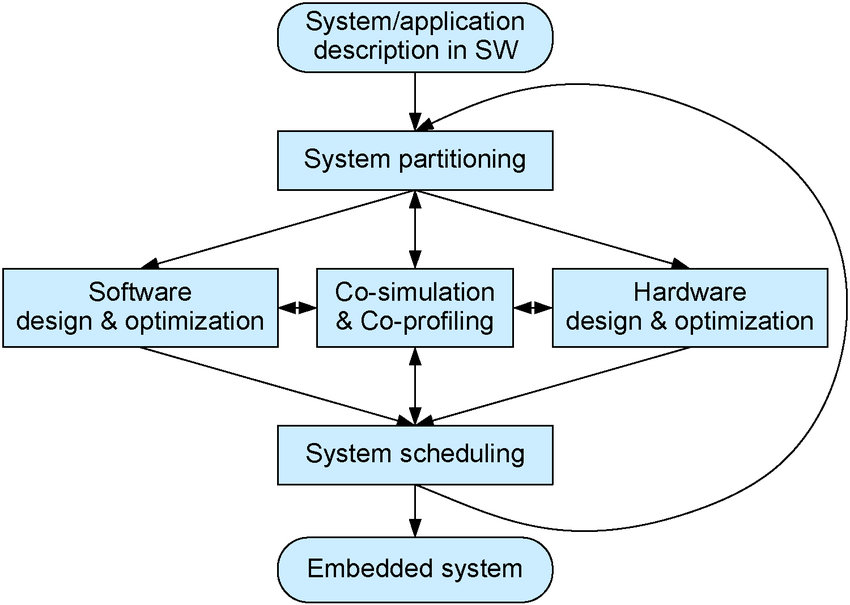
\includegraphics[width=0.5\textwidth]{images/embedded_sys_df.png}
	\caption{Flusso di progettazione di un sistema embedded.}
	\label{pse}
\end{figure}

Fatta questa premessa, ci si vuole ora concentrare sulla parte di sintesi hardware che può essere fatta in solo due modi. Il primo, previsto dall'attuale stato dell'arte, prevede la traduzione manuale del codice software in una descrizione hardware. Ciò garantisce, ovviamente, un maggiore controllo sul risultato finale. Il secondo metodo consiste invece di affidarsi a tool automatici per l'\emph{high level synteshis} che risulta essere molto più veloce ma anche meno controllabile nella qualità del risultato. Come già mostrato in figura \ref{hls}, il processo di HLS prevede una serie di fasi per poter ottenere una descrizione hardware a partire da un codice sorgente. Tra questa fasi sicuramente la più importante è quella che riguarda lo \emph{scheduling} (anche se in figura scheduling e resource alloaction condividono la stesso posto nel diagramma, lo stato dell'arte prevede che prima venga fatto lo scheduling e solo in un secondo momento vengano allocate le risorse in base al risultato precedentemente ottenuto, motivo per cui in questa relazione si parlerà esclusivamente di scheduling e mai di resource allocation).

La fase di scheduling consiste fondamentalmente in tre passaggi con tre algoritmi diversi applicati in sequenza:
\begin{itemize}
	\item  Scheduling ASAP: Lo scheduling ASAP è il primo passa per trasformare un DFG in un grafo temporizzato. Con questo algoritmo si impone che tutte le operazioni dei nodi vengano fatte nel primo tempo utile senza infrangere nessun vincolo, andando così a determinare il valore dell'attributo $t$ dei nodi del TG risultante ed ottenendo di conseguenza il minimo numero di cicli impiegati dal circuito 
	\item Scheduling ALAP: Lo scheduling ALAP riceve come input il risultato del precedente algoritmo ed esegue l'operazione diametralmente opposta, poiché viene imposto che tutte le operazioni dei nodi vengano eseguite nell'ultimo tempo utile senza infrangere nessun vincolo ed andando così a determinare il valore dell'attributo $T$ di tutti i nodi del grafo risultato.
	\item Fase di ricerca: Una volta ottenuti i valori di tempo minimo e massimo per ogni nodo incomincia una fase di ricerca in cui vengono spostati tutti i nodi con lo scopo di andare a minimizzare una data funzione di costo (in questa relazione la funzione di costo è data dal numero di nodi che lavorano in parallelo, ovvero dal numero di nodi che operano allo stesso tempo).
\end{itemize}
Le figure \ref{scheduling} e \ref{scheduling2} mostrano un esempio dell'applicazione di quanto riportato sopra.
\begin{figure}[htp]
	\centering
	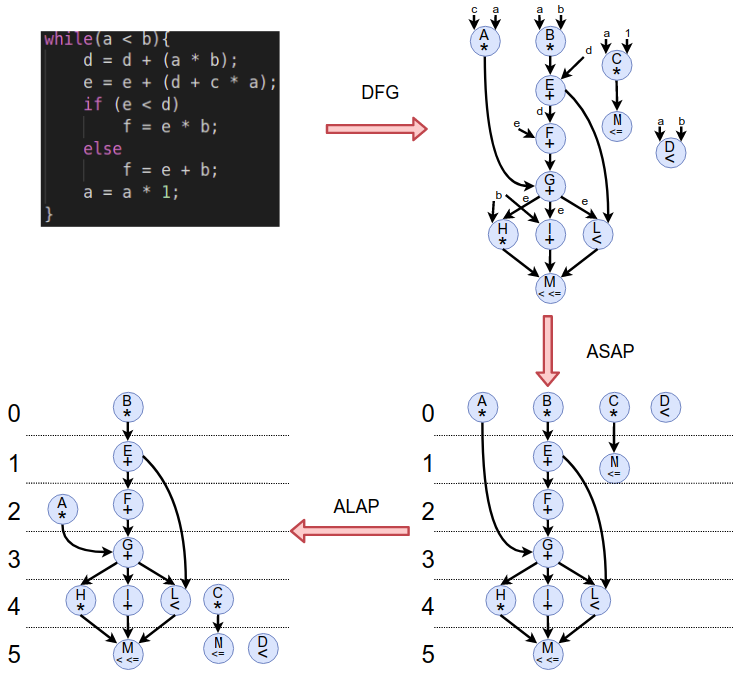
\includegraphics[width=0.5\textwidth]{images/schedule.png}
	\caption{Trasformazione di un codice sorgente in DFG e applicazione degli algoritmi ASAP e ALAP (le variabili usate nei nodi sono state omesse dopo lo scheduling asap).}
	\label{scheduling}
\end{figure}
\begin{figure}[htp]
	\centering
	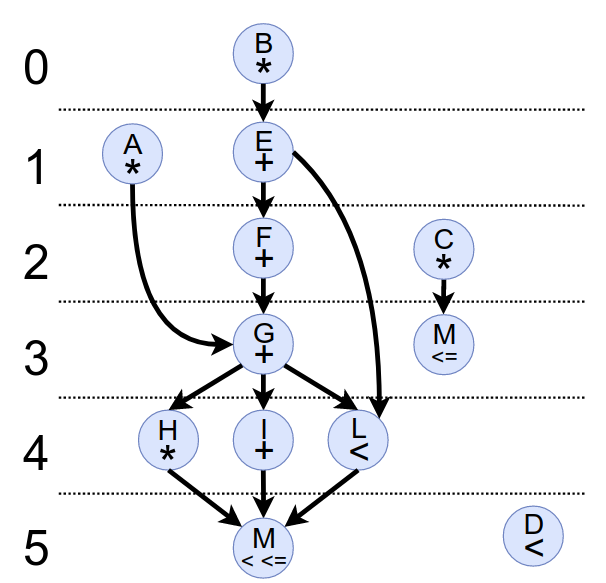
\includegraphics[width=0.3\textwidth]{images/scheduling2.png}
	\caption{Possibile risultato  dello scheduling (permutazione del grafo) applicato al codice della figura \ref{scheduling}}
	\label{scheduling2}
\end{figure}


In questa relazione si proporrà quindi un algoritmo che, sfruttando l'approccio distribuito basato su map-reduce e le funzionalità del framework Hadoop, cercherà di dare una soluzione ottima al problema della ricerca del grafo ottimo.
\section{Approccio al problema}
Definito il problema, si può passare ora a descrivere l'approccio usato per risolverlo.

Il primo passo fatto è stato quello di andare ad inquadrare il problema in un contesto di tipo map-reduce andando quindi a mappare le fasi che l'algoritmo prevede su quelle del paradigma usato, riservandosi anche di effettuare più cicli di map-reduce qualora necessario.
\subsection{Trasposizione in Map-Reduce}
Trasporre il problema in modo da adattarlo al paradigma map-reduce non è un'operazione complicata. Supponendo di ricevere come input già un DFG, le uniche fasi da implementare sono i tre algoritmi di scheduling, due dei quali tuttavia, ovvero ASAP e ALAP, possono essere applicati in sequenza e non richiedono troppe risorne nè di computazione nè di tempo. La parte più onerosa in termini di costo di computazione riguarda infatti la fase di ricerca dove è necessario andare ad esplorare tutti i possibili grafi validi e calcolare il costo di ognuno, ed è quindi questa fase che si vuole andare ad ammortizzare tramite il calcolo distribuito. 

Per ottenere questo risultato si è partiti da una prima idea di soluzione, ovvero di distribuire l'onere del calcolo delle varie permutazioni tra le varie macchine del cluster, e la si è andata a raffinare e modificare lungo tutto il corso del lavoro. Di seguito sono riportate le tre fasi principali cui la soluzione è andata incontro.
\begin{itemize}
	\item Fase 1 (fig.\ref{sol_fase1}): In questa prima fase la soluzione consiste essenzialmente in tre passaggi distinti. In un primo passaggio il DFG è processato da un'unica unità centrale con lo scopo di andare a calcolare le varie permutazioni dello stesso. Successivamente queste permutazioni sono inviate ai vari mapper che procedono a calcolarne il costo ed a inviarlo ad un unico reducer che cerca la soluzione a costo migliore. Ovviamente il fatto di dover calcolare tutte le permutazioni in un'unica entità centrale non ha garantito buone prestazioni e ciò a fatto sì che la soluzione venisse migliorata nella seconda fase.
	
	\item Fase 2 (fig.\ref{sol_fase2}): Questa fase mantiene lo scheletro della precedente ma sposta il calcolo delle permutazioni sui mapper. Adesso l'unità centrale deve solamente stimare il numero di permutazioni che possono essere generate, dividere tale numero per il numero di macchine presenti e dire ai mapper quante permutazioni calcolare e da quale partire (per maggiori dettagli si veda la sezione \ref{stima}). Di conseguenza in questa fase si ha un potenziamento dei mapper che devono non solo calcolare tutta una serie di permutazioni di un grafo (eliminando eventuali comfigurazioni illegali) ma per ognuna di queste deve anche calcolarne il relativo costo da inviare al reducer che, rispetto alla fase precedente, non ha subito essenziali modifiche. Già con queste modifiche la soluzione si presenta più performante rispetto alla precedente ma, a causa della struttura con cui hadoop è creato, non è implementabile. Si è dovuto quindi effettuare una seconda ristrutturazione per rendere la soluzione compatibile con il framework.

	
	\item Fase 3 (fig.\ref{sol_fase3}): Questa fase, seppur mantenendo i concetti espressi nella seconda, vede uno shift a livello di passaggi coinvolti. Adesso infatti l'unità centralizzata responsabile del calcolo delle permutazioni viene completamente eliminata e le sue funzionalità sono ereditate da un singolo mapper che calcola il punto di partenza e il numero di permutazioni da inviare ai reducer. Questi infatti ereditano le funzionalità dei mapper e devono calcolare la migliore permutazione tra tutte quelle loro assegnate. Ciò comporta che l'output del job non è più un unico grafo come in precedenza ma una numero di grafi pari al numero di reducer ed è quindi necessario un modo per cercare il migliore. Questo può essere fatto tramite un semplice job di map-reduce oppure (in caso di un numero ristretto di output) con un semplice programma sequenziale.
	\begin{figure}[htp]
		\centering
		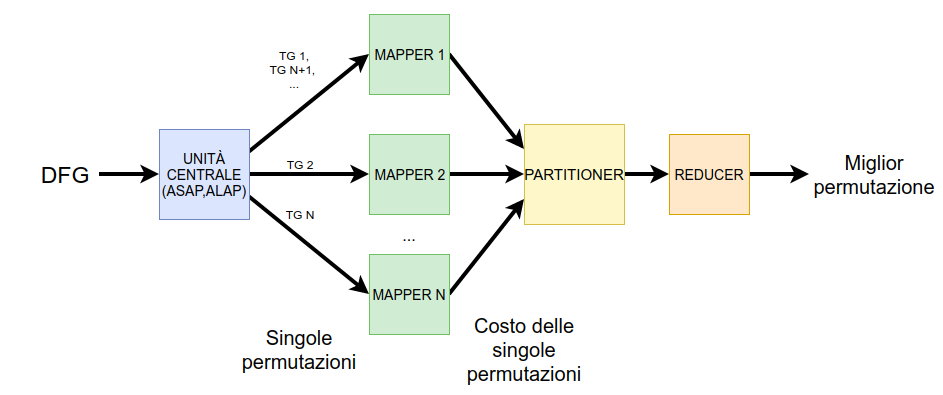
\includegraphics[width=0.5\textwidth]{images/sol_fase1.png}
		\caption{Schema della soluzione nella prima fase.}
		\label{sol_fase1}
		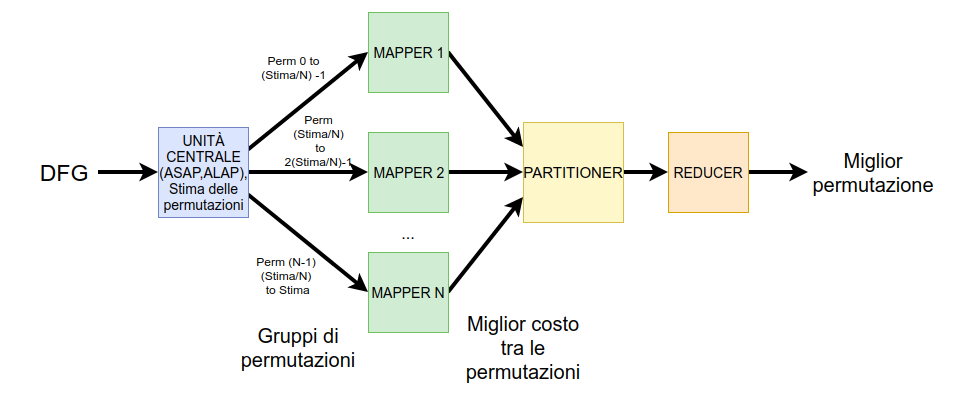
\includegraphics[width=0.5\textwidth]{images/sol_fase2.png}
		\caption{Schema della soluzione nella seconda fase.}
		\label{sol_fase2}
		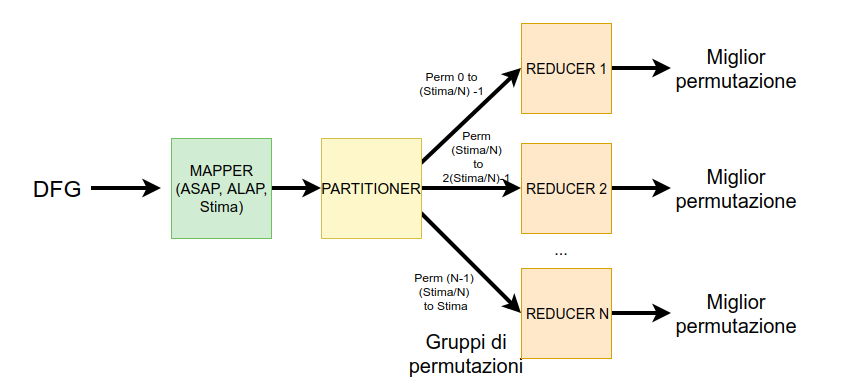
\includegraphics[width=0.5\textwidth]{images/sol_schema3.png}
		\caption{Schema della soluzione nella terza fase.}
		\label{sol_fase3}
	\end{figure}

	
\end{itemize}
\subsection{Implementazione con Hadoop}
Dopo aver definito lo schema della soluzione da adottare si è passati all'effettiva implementazione in Hadoop. Poiché il framework supporta pienamente il paradigma map-reduce è stato sufficiente andare ad implementare le varie classi necessarie perché il job venisse accettato, ovvero le classi java \emph{Driver}, \emph{InputReader}, \emph{Mapper}, \emph{Partitioner} e \emph{Reducer} (approfondite nella sezione \ref{work}). Se l'implementazione delle classi è stata facile, ci si è dovuti però andare a scontrare con alcune delle limitazioni imposte dal framework, limitazioni che in più punti hanno costretto a modificare la soluzione adottata o ad imporre delle restrizioni in modo forzato.

La prima limitazione incontrata è dovuta all'impossibilità di conoscere a runtime il numero di nodi che il cluster possiede. Senza questa informazione non si sarebbe potuto suddividere le permutazioni tra le macchine e, di conseguenza, non sarebbe stato possibile risolvere il problema nel modo desiderato. Per porre rimedio a ciò si è scelto di imporre all'utente di inserire, al lancio del job, la granularità del parallelismo voluto, ovvero il numero per cui le permutazioni stimate vanno divise e quindi la quantità di lavoro assegnata ad ogni singolo nodo. Sebbene in un primo momento questa scelta possa sembrare una limitazione eccessiva, una volta implementata la terza soluzione, ci si è resi conto che venivano introdotti come effetto collaterale due importanti vantaggi. Con questo metodo è possibile, in primo luogo, scegliere di non usare tutta la potenza di calcolo del cluster ma solo una frazione, lasciando liberi gli altri nodi di eseguire altri job. In seconda istanza si può, al contrario di prima, andare ad inserire un valore che supera il numero di nodi nel cluster. In questo modo ogni nodo si troverà a dover eseguire un numero minore di operazioni e, di conseguenza, i nodi più veloci riusciranno a completare più task di reduce rispetto a quelli lenti che faticano a completarne uno. Grazie a ciò si crea un meccanismo semi-automatico del bilanciamento del carico di lavoro al prezzo di un aumento del numero dei file di output (ogni task di reduce genera un file di output).
\begin{figure}
	\centering
	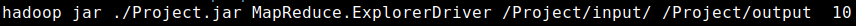
\includegraphics[width=0.5\textwidth]{images/exec.png}
	\caption{Comando per lanciare il job su Hadoop. Si noti il numero ``10'' posto alla fine ad indicare di dividere le permutazioni per 10 cluster. Inoltre se possibile verranno usati 10 nodi per eseguire i task di reduce (in caso il numero sia eccessivo Hadoop allocherà quanto disponibile senza ritornare errore).}
\end{figure}

Un'altro ostacolo incontrato durante l'implementazione del software è stato la difficoltà con cui Hadoop permette di scegliere il numero di mapper da usare. Se infatti Hadoop permette in modo molto facile di manipolare il numero di reducer usati, il modo in cui il numero di mapper è calcolato è difficilmente influenzabile dal programmatore. Questo è dovuto al fatto che il framework, per come è stato concepito, si aspetta di processare in input o un'unico file di grandi dimensioni oppure diversi file in quanto, sostanzialmente, il numero di mapper è calcolato come la somma delle dimensioni in byte di tutti i file diviso una data costante. Tuttavia nel nostro caso capita sempre che i file usati come input e contenenti il DFG iniziale siano sempre troppo piccoli rispetto alla costante impostata e di conseguenza si ottiene sempre l'allocazione di un solo mapper. Per risolvere questo problema si sono applicate due diverse soluzioni a seconda della fase della soluzione in cui si stava lavorando. Nella prima e seconda fase ciò che è stato fatto è stato di andare a manipolare la costante usata nella divisione impostandola al rapporto tra la dimensione totale dell'input, letta precedentemente, e il numero di mapper voluto. In questo modo il valore del numero di mapper che Hadoop imposta era esattamente il valore voluto.

Nel momento in cui si è passati alla terza fase della soluzione questo procedimento non era però più necessario in quanto ora bisognava solo accertarsi che il mapper allocato fosse esattamente uno. Dopo un'attenta analisi del codice di Hadoop, in particolare la parte riguardante la classe \emph{FileInputFormat}\cite{FILEINPUTFORMAT} e \emph{JobConf}\cite{JOBCONF} si è potuto notare come il numero di mapper sia calcolato da Hadoop. Molto semplicemente il framework prende ogni file in input, verifica se è possibile fare lo split e, se possibile, lo divide ed inserisce le partizioni all'interno di un'apposita lista, altrimenti il file non viene diviso ma comunque viene aggiunto un elemento all'interno della lista precedentemente citata. La dimensione di tale lista è poi usata da Hadoop per allocare i mapper. Ciò che è stato fatto quindi è stato solamente andare a sovrascrivere il metodo booleano per il controllo dello splitting andando a fare in modo che ritornasse sempre il valore \texttt{false}. In questa maniera, e poiché il software accetta solo un file in input, sia che l'input sia troppo piccolo o troppo grande nella lista degli split verrà inserita una ed una sola entry e di conseguenza verrà allocato solo un mapper.

Ultimo ostacolo affrontato è stato il modo in cui il framework gestisce la suddivisione degli input. Come si è potuto osservare in precedenza, sia la prima che la seconda fase della soluzione proposta si basavano fortemente sull'uso di un nodo centrale per il parsing e la suddivisione dei grafi tra i mapper. Inizialmente si era pensato di affidare il compito alla classe responsabile di leggere il file di input nell'errata convinzione che questa fosse univoca all'interno del framework. Dopo alcuni test e ricerche si è però capito che in realtà questa classe non è unica rispetto al framework ma è univoca rispetto al mapper, ovvero ogni mapper istanzia una classe propria che legge l'input, anch'esso replicato sulle diverse macchine. A causa di ciò il lavoro che doveva essere fatto solo una volta veniva moltiplicato per il numero di mapper allocati, rompendo quindi la correttezza del programma. A causa di ciò si è deciso di modificare il programma, passando dunque alla terza fase, e di delegare il compito della suddivisione delle partizioni al mapper, il quale può essere univoco all'interno del framework.
\begin{figure}
	\centering
	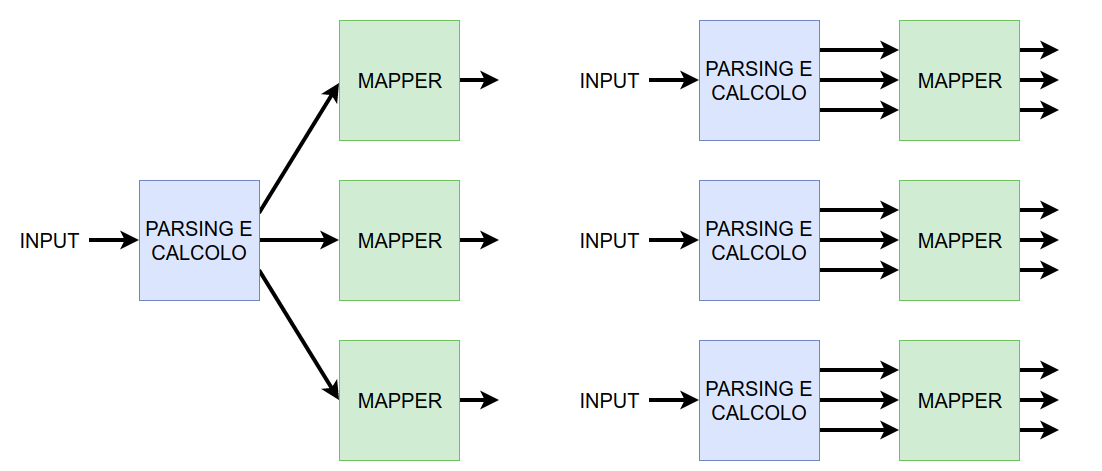
\includegraphics[width=0.5\textwidth]{images/hadoop_input.png}
	\caption{A sinistra il modo in cui l'input doveva essere processato secondo la soluzione nella sua prima e seconda fase, a destra il modo in cui Hadoop lo gestiva. Si noti che in questo modo ogni mapper esegue tutto il lavoro e non solo una porzione.}
\end{figure}

\section[Lavoro]{Lavoro svolto \footnote{Codice sorgente completo reperibile a \url{https://github.com/brentelia/HLS-scheduling-distributed-solver}}} \label{work}
Per implementare soluzione proposta tramite Hadoop è stato sufficiente andare ad implementare tutte le classi che il framework richiede per poter sottomettere un job  di map-reduce al cluster. Di seguito sono riportate tutte le classi implementate con le relative spiegazioni e porzioni di codice.
\subsection{Classe Driver}
In un job di Hadoop la classe \emph{Driver} ha il compito di andare a preparare  l'ambiente in cui l'applicazione verrà lanciata andando configurare tutte le variabili necessarie. La classe Driver implementata nel software proposto non si distacca da questa molto da questo paradigma ma presenta comunque alcuni punti degni di nota.

Il primo punto importante riguarda i parametri in input. Normalmente un'applicazione Hadoop prevede come input solamente il path per l'input e quello per l'output ma nel nostro caso è stato aggiunto un terzo parametro, ovvero il livello di parallelismo voluto, che deve quindi essere letto e inserito all'interno di una variabile di ambiente in modo che poi possa essere recuperato successivamente nel mapper dato che non è possibile alcun tipo di comunicazione diretta tra la classe driver e le altri classi del framewrok.
\begin{lstlisting}[style=javaStyle]

	if (args.length != 3) {
		System.err.println("Usage: ExplorerDriver <input path> <outputpath> <#_nodes_to_use>");
		System.exit(-1);
	}
	...
	//set number of reducers by casting 3rd agument
	int nodes=Integer.parseInt(args[2]);
	//set the variabile "nodes" in the job configuration class
	conf.setInt("nodes", nodes);
\end{lstlisting}

Secondo punto degno di nota è dato dal fatto che il Driver ha il compito di andare ad indicare al framework tutte le classi utili per lo svolgimento del programma così come il tipo dei dati prodotti in output ed il numero di reducer usati:
\begin{lstlisting}[style=javaStyle]
//number of reducers
jobConf.setNumReduceTasks(nodes); 
...
//job name displayed
job.setJobName("Graph Exploration"); 
...
//Iinput path of the file
FileInputFormat.addInputPath(job, new Path(args[0])); 
//Input parser class
job.setInputFormatClass(
	GraphInputFormat.class); 
//Output directory
FileOutputFormat.setOutputPath(job, new Path(args[1]));
//Mapper class
job.setMapperClass(ExplorerMapper.class);	
//Reducer class
job.setReducerClass(ExplorerReducer.class); 
//Partitioner class
job.setPartitionerClass(
	ExplorerPartitioner.class); 
//Key and Value types
job.setOutputKeyClass(Text.class); 
job.setOutputValueClass(Text.class);
\end{lstlisting}
\subsection{Classe GraphInputReader}
La classe GraphInputReader è una classe che estende l'originaria classe RecordReader di Hadoop. Tale classe aveva, in origine, lo scopo di leggere porzioni di file da inviare al mapper associatogli (tipicamente riga per riga) fino all'esaurimento del file in input. Tuttavia poiché questo comportamento non si adattava bene a quello del programma è stato scelto di sostituirla con una classe apposita con lo scopo di leggere in un unico colpo tutto il file. Per poter fare questo si è andati a modificare il metodo \emph{initialize} ereditato dalla classe padre in modo da salvare tutto il file all'interno di una stringa che viene poi inviata come coppia chiave-valore (la chiave è una stringa vuota) al mapper. Dopo il primo invio del grafo, una flag viene settata in modo che la funzione ereditata \emph{nextKeyValue()}, metodo cui scopo è far sapere l'eventuale presenza di ulteriori dati da inviare, ritorni il valore \texttt{false} così che il mapper non faccia richiesta di ulteriori dati. Di seguito è riportato un esempio di un file di input riferito al DFG in figura \ref{scheduling}. 
\VerbatimInput{files/DAG.txt}
All'interno del file ogni riga descrive un nodo del grafo con: \texttt{nome:operatore/nodi\_input/nodi\_output}.


\subsection{Mapper}\label{stima}
Il Mapper è responsabile di:
\begin{itemize}
	\item eseguire il parse del grafo;
	\item calcolare la mobilità di ogni nodo;
	\item stimare il numero di permutazioni;
	\item creare le mappature per distribuire il calcolo.
\end{itemize}
Il mapper riceve come input la stringa contenente il grafo ed è quindi necessario costruire una struttura dati appropriata per poterlo gestire. Questo viene realizzato tramite l'utilizzo di una HashMap che permette una associazione in $O(1)$ tra il nome del nodo (come rappresentato nel file di input) e l'effettiva struttura dati contenente tutti i dati del nodo stesso. Questo permette il parse del grafo in tempo $O(V+E)$, dal momento che è necessario esplorare anche tutti gli archi per trovare i nodi padri/figli di ogni nodo. Oltre a ciò vengono anche eseguiti gli scheduling ASAP e ALAP sul grafo in modo da calcolare gli attributi $t$, $T$ e della mobilità $m$, necessari al calcolo delle permutazioni successive.

Calcolare ogni possibile permutazione del grafo è un'operazione estremamente pesante in termini di tempo ($O(V!)$), ma è necessario per poter suddividere il carico di lavoro tra i vari Reducer. Per cercare quindi di ridurre la complessità del calcolo si è  deciso di andare sovrastimare il numero di possibili permutazioni (aggiungendo quindi combinazioni invalide) ma riuscendo ad eseguire questa stima in tempo lineare $O(V+E)$, garantendo quindi la possibilità di analizzare anche grafi molto grandi. Questa stima viene realizzata analizzando delle strutture presenti nel grafo che qui chiameremo \emph{catene}. Una catena è definita come un insieme di nodi aventi la stessa mobilità (attributo $m$) e dove ogni nodo (eccetto uno) possiede uno e un solo figlio nella catena.

\begin{figure}[htp]
	\centering
	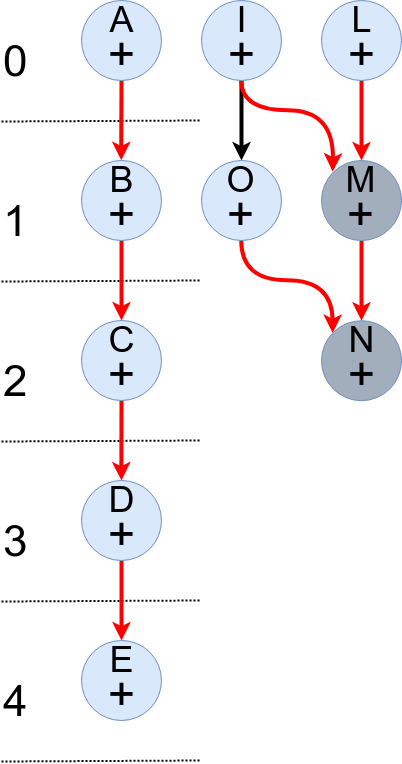
\includegraphics[height=0.25\textheight]{images/chains.png}
	\caption{Due esempi di catene di nodi. A destra vi è una situazione in cui le catene potrebbero generare errori. I due nodi scuri potrebbero essere inseriti in più catene diverse e perderebbero la loro dipendenza dall'altro nodo. In questo caso le catene possibili sarebbero N-O-I e M-L, N-M-L e O-I, N-M-I e due nodi singoli O e L. }
\end{figure}

L'introduzione del concetto di catena è fondamentale per il calcolo delle permutazioni poiché per ogni una di queste è facile calcolare le possibili permutazioni in quanto una catena di $x$ nodi e $m$ mobilità ha permutazioni pari a $P_{x+m}^{x,m} = \frac{(x+m)!}{x!m!}$
\'E tuttavia possibile che alcuni nodi facciano però parte di più possibili catene: in questo caso il nodo viene inserito nella catena più lunga, introducendo tuttavia un errore in quanto una possibile dipendenza temporale verrebbe nascosta ed inserendo quindi permutazioni non valide nel pool da testare.

Infine la stima totale viene ottenuta moltiplicando tra loro le permutazioni possibili di ogni catena presente nel grafo.

Una volta finita la stima il mapper mappa le permutazioni tra i Reducer specificati dall'utente, dividendo le permutazioni equamente tra tutti, specificando i nodi componenti di ogni catena, il numero della permutazione iniziale e l'ammontare di permutazioni da calcolare.
\begin{figure}[htp]
	\centering
	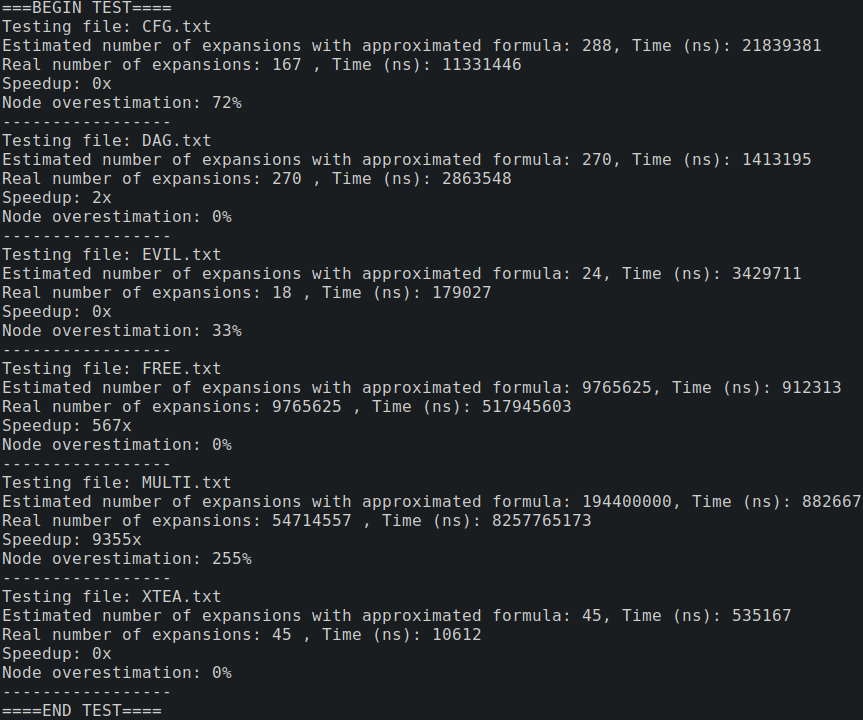
\includegraphics[width=0.45\textwidth]{images/tests.png}
	\caption{Alcuni test eseguiti su diversi file con diversi grafi. L'immagine mostra per ogni test il tempo impiegato per stimare le permutazioni dei grafi e il tempo effettivo per poterle calcolare tutte. Inoltre sono riportati lo speedup ottenuto e la percentuale la sovrastima in percentuale.}
\end{figure}

\subsection{Classe Partitioner}
La classe \emph{Partitioner} ha il compito, all'interno del framework, di andare a distribuire i risultati dei mapper tra i vari reducer. Tipicamente questo è fatto andando a creare l'hash delle chiave usando il resto della divisione per il numero di reducer come identificativo del reducer cui il dato deve essere girato. In questo caso però ciò non è necessario poiché il numero di risultati è esattamente uguale al numero di reducer usati, quindi ogni risultato è mappato univocamente su un solo reducer tramite un semplice contatore che va da 0 al numero di questi meno uno.
\begin{lstlisting}[style=javaStyle]
public class ExplorerPartitioner extends Partitioner<Text,Text>{

	private Integer counter;
	@Override
	public int getPartition(Text key, Text val, int partitions) {
		return (counter == null ? counter = 0 : ++counter);
	}
}
\end{lstlisting}

\subsection{Reducer}
Il compito più importante all'interno dell'applicazione spetta al reducer. Questo deve:
\begin{itemize}
	\item eseguire il parse del grafo ricevuto in input;
	\item eseguire il parse delle catene;
	\item calcolare la posizione iniziale del grafo;
	\item analizzare ogni permutazione assegnata;
	\item restituire la combinazione migliore.
\end{itemize}
Le prime due operazioni possono essere svolte con relativa facilità in quanto si tratta solo di andare a ritrovare nella stringa inviata dal mapper tutti i vari dati che sono utili per poter eseguire il calcolo. In particolare le catene sono inserite in strutture dati apposite dotate di metodi utili per i futuri calcoli. 
Il calcolo della posizione iniziale del grafo (ovvero la configurazione da cui calcolare le permutazioni successive) comincia con il calcolo della \emph{base} di ogni catena, ossia il numero di permutazioni ammesse all'interno della catena stessa. Sapendo dunque che la stima è stata ottenuta come prodotto delle possibili permutazioni di ogni catena è quindi possibile fattorizzarla usando gli stessi valori (ossia le basi). Il numero ricevuto come permutazione iniziale viene perciò fattorizzato usando le basi di ogni catena, permettendo di ottenere il numero della permutazione relativa ad ogni singola catena necessario per ottenere la configurazione iniziale. Avendo ottenuto il numero di permutazione per ogni catena, vengono calcolate la permutazioni (e di conseguenza, posizione temporale dei nodi al loro interno) associate, ottenendo così la posizione di partenza del grafo da analizzare.
\begin{figure}[htp]
	\centering
	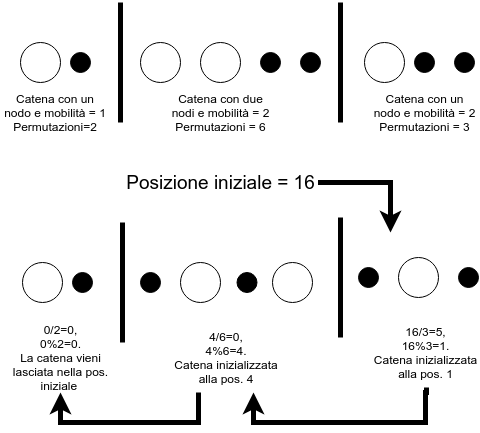
\includegraphics[width=0.5\textwidth]{images/fact.png}
	\caption{Esempio di fattorizzazione. Il grafo è composto da tre catene, rappresentate da nodi chiari (i nodi del grafo) e nodi scuri (gli spazi occupabili nel tempo dai nodi). L'immagine mostra come la posizioni iniziale 16 è tradotta nelle varie posizioni dei nodi nel grafo}
\end{figure}

In seguito per ogni permutazione ne viene analizzata la validità, controllando quindi eventuali violazioni di vincoli temporali (che, come specificato in precedenza, possono esistere). Nel caso il grafo in analisi risulti essere valido ne viene controllato il costo e, se risulta migliore del risultato parziale, lo sostituisce. 
In questo progetto si è utilizzato come funzione di costo il massimo numero di nodi paralleli tra loro, e come obiettivo la minimizzazione dello stesso.
Una volta finito il passaggio precedente si incrementa il numero della permutazione da analizzare, incrementando il valore della catena "meno significativa" all'interno del numero e propagando eventuali riporti verso le altre catene, ricalcolando poi la posizione relativa di ogni nodo al loro interno.
Questo metodo permette di calcolare ogni permutazione successiva modificando il minor numero di nodi possibile e minimizzando quindi la complessità dell'algoritmo.
Finita la valutazione di ogni permutazione il Reducer manda quindi il risultato in output.
Non sempre, però, questo è da considerarsi valido, in quanto in alcuni casi ( quando il numero di Reducer assegnati è troppo grande per il numero di permutazioni da calcolare) è possibile arrivare al termine dell'analisi senza aver mai trovato un grafo valido. In questi casi viene comunque ritornata la posizione iniziale assegnata, ma ne viene specificata la sua non validità.

\section{Risultati ottenuti}
Dopo aver completato l'algoritmo e averlo testato in locale si è passato al test su cluster. 
Nel particolare è stato usato un cluster composto da dieci nodi diversi sui quali sono stati lanciati in sequenza molteplici file di test tramite un apposito script bash creato per andare a lanciare in successione diversi job con input sempre diversi e per collezionare in un file di log tutti gli output del framework e le statistiche relative ai tempi impiegati. La tabella \ref{results} mostra i risultati dei vari test, tutti i quali sono stati svolti ponendo come livello di parallelismo il valore 100 (e di conseguenza producendo cento file di output).

 \begin{table}[htp]
	\resizebox{\columnwidth}{!}{
	\begin{tabular}{l r r r r}
		\toprule
		\multicolumn{1}{c}{File di test}&\multicolumn{1}{r}{Permutazioni valide}&\multicolumn{1}{c}{Permutazioni valutate} & \multicolumn{1}{c} {Tempo impiegato (m:s)} \\
		\midrule
		DAG.txt 	& 270		& 270	 	& 1:6.582\\
		CFG.txt 	& 167	 	& 288	 	& 1:8.647\\
		XTEA.txt 	& 45	 	& 45	 	& 1:6.673\\
		FREE.txt	&9765625	& 9765625	& 1:18.74\\
		EVIL.txt	& 18		& 24		& 1:2.505\\
		MULTI.txt	&54714557	&194400000	& 8:11.72\\
		\bottomrule
	\end{tabular}
	}
	\caption{Relazione tra numero di permutazioni del grafo e tempo impiegato dal cluster (valori riferiti ad una granularità del parallelismo pari a 100).}
	\label{results}
\end{table}
Come si può notare dalla tabella riportata, l'algoritmo implementato riesce tranquillamente a gestire grafi con milioni di permutazioni possibili utilizzando una stima abbastanza precisa e trovando i risultati migliori in tempi molto brevi. Tra tutti i risultati ottenuti è inoltre garantita la presenza di almeno una soluzione ottima, in quanto è possibile che più reducer producano una soluzione a costo minimo. La soluzione voluta va quindi cercata tra tutte quelle che presentano il costo minimo.
\section{Conclusioni}

Il problema dello scheduling è sicuramente una delle problematiche più difficili che bisogna affrontare nel momento in cui si vuole andare ad affrontare un problema di high level synthesis. Ovviamente la ricerca della configurazione migliore tra milioni di possibili non è sempre ottenibile in modo facile in quanto il problema stesso appartiene alla classe \emph{NP}. A causa di ciò al momento non è possibile dare una soluzione ottima al problema senza pagare un prezzo in tempo a volte anche molto alto. La soluzione qui proposta tenta quindi di andare ad abbassare i limiti di tempo attuali sfruttando la potenza combinata non di una ma di più macchine che lavorano parallelo. In questo modo sebbene non sarà possibile risolvere realmente il problema in questione si sarà comunque in grado di risolvere problemi complessi non risolvibili su singoli calcolatori, sfruttando la potenza di cluster sempre più potenti e grandi.

\bibliographystyle{IEEEtran}
\bibliography{biblio}

\end{document}